%%%%%%%%%%%%%%%%%%%%%%%%%%%%%%%%%%%%%%%%%
% Programming/Coding Assignment
% LaTeX Template
%
% This template has been downloaded from:
% http://www.latextemplates.com
%
% Original author:
% Ted Pavlic (http://www.tedpavlic.com)
%
% Note:
% The \lipsum[#] commands throughout this template generate dummy text
% to fill the template out. These commands should all be removed when 
% writing assignment content.
%
% This template uses a Perl script as an example snippet of code, most other
% languages are also usable. Configure them in the "CODE INCLUSION 
% CONFIGURATION" section.
%
%%%%%%%%%%%%%%%%%%%%%%%%%%%%%%%%%%%%%%%%%

%----------------------------------------------------------------------------------------
%	PACKAGES AND OTHER DOCUMENT CONFIGURATIONS
%----------------------------------------------------------------------------------------

\documentclass{article}

\usepackage{fancyhdr} % Required for custom headers
\usepackage{lastpage} % Required to determine the last page for the footer
\usepackage{extramarks} % Required for headers and footers
\usepackage[usenames,dvipsnames]{color} % Required for custom colors
\usepackage{graphicx} % Required to insert images
\usepackage{subcaption}
\usepackage{listings} % Required for insertion of code
\usepackage{courier} % Required for the courier font
\usepackage{lipsum} % Used for inserting dummy 'Lorem ipsum' text into the template
\usepackage{amsmath} % Use for multiple line equations
\usepackage{color}
% Margins
\topmargin=-0.45in
\evensidemargin=0in
\oddsidemargin=0in
\textwidth=6.5in
\textheight=9.0in
\headsep=0.25in

\linespread{1.1} % Line spacing

% Set up the header and footer
\pagestyle{fancy}
\lhead{\hmwkAuthorName} % Top left header
\chead{\hmwkClass\ (\hmwkClassTime): \hmwkTitle} % Top center head
%\rhead{\firstxmark} % Top right header
\lfoot{\lastxmark} % Bottom left footer
\cfoot{} % Bottom center footer
\rfoot{Page\ \thepage\ of\ \protect\pageref{LastPage}} % Bottom right footer
\renewcommand\headrulewidth{0.4pt} % Size of the header rule
\renewcommand\footrulewidth{0.4pt} % Size of the footer rule

\setlength\parindent{0pt} % Removes all indentation from paragraphs

%----------------------------------------------------------------------------------------
%	CODE INCLUSION CONFIGURATION
%----------------------------------------------------------------------------------------

\definecolor{MyDarkGreen}{rgb}{0.0,0.4,0.0} % This is the color used for comments
\lstloadlanguages{Perl} % Load Perl syntax for listings, for a list of other languages supported see: ftp://ftp.tex.ac.uk/tex-archive/macros/latex/contrib/listings/listings.pdf
\lstset{language=Perl, % Use Perl in this example
        frame=single, % Single frame around code
        basicstyle=\small\ttfamily, % Use small true type font
        keywordstyle=[1]\color{Blue}\bf, % Perl functions bold and blue
        keywordstyle=[2]\color{Purple}, % Perl function arguments purple
        keywordstyle=[3]\color{Blue}\underbar, % Custom functions underlined and blue
        identifierstyle=, % Nothing special about identifiers                                         
        commentstyle=\usefont{T1}{pcr}{m}{sl}\color{MyDarkGreen}\small, % Comments small dark green courier font
        stringstyle=\color{Purple}, % Strings are purple
        showstringspaces=false, % Don't put marks in string spaces
        tabsize=5, % 5 spaces per tab
        %
        % Put standard Perl functions not included in the default language here
        morekeywords={rand},
        %
        % Put Perl function parameters here
        morekeywords=[2]{on, off, interp},
        %
        % Put user defined functions here
        morekeywords=[3]{test},
       	%
        morecomment=[l][\color{Blue}]{...}, % Line continuation (...) like blue comment
        numbers=left, % Line numbers on left
        firstnumber=1, % Line numbers start with line 1
        numberstyle=\tiny\color{Blue}, % Line numbers are blue and small
        stepnumber=5 % Line numbers go in steps of 5
}

% Creates a new command to include a perl script, the first parameter is the filename of the script (without .pl), the second parameter is the caption
\newcommand{\perlscript}[2]{
\begin{itemize}
\item[]\lstinputlisting[caption=#2,label=#1]{#1.pl}
\end{itemize}
}

%----------------------------------------------------------------------------------------
%	DOCUMENT STRUCTURE COMMANDS
%	Skip this unless you know what you're doing
%----------------------------------------------------------------------------------------

% Header and footer for when a page split occurs within a problem environment
\newcommand{\enterProblemHeader}[1]{
%\nobreak\extramarks{#1}{#1 continued on next page\ldots}\nobreak
%\nobreak\extramarks{#1 (continued)}{#1 continued on next page\ldots}\nobreak
}

% Header and footer for when a page split occurs between problem environments
\newcommand{\exitProblemHeader}[1]{
%\nobreak\extramarks{#1 (continued)}{#1 continued on next page\ldots}\nobreak
%\nobreak\extramarks{#1}{}\nobreak
}

\setcounter{secnumdepth}{0} % Removes default section numbers
\newcounter{homeworkProblemCounter} % Creates a counter to keep track of the number of problems
\setcounter{homeworkProblemCounter}{-1}

\newcommand{\homeworkProblemName}{}
\newenvironment{homeworkProblem}[1][Part \arabic{homeworkProblemCounter}]{ % Makes a new environment called homeworkProblem which takes 1 argument (custom name) but the default is "Problem #"
\stepcounter{homeworkProblemCounter} % Increase counter for number of problems
\renewcommand{\homeworkProblemName}{#1} % Assign \homeworkProblemName the name of the problem
\section{\homeworkProblemName} % Make a section in the document with the custom problem count
\enterProblemHeader{\homeworkProblemName} % Header and footer within the environment
}{
\exitProblemHeader{\homeworkProblemName} % Header and footer after the environment
}

\newcommand{\problemAnswer}[1]{ % Defines the problem answer command with the content as the only argument
\noindent\framebox[\columnwidth][c]{\begin{minipage}{0.98\columnwidth}#1\end{minipage}} % Makes the box around the problem answer and puts the content inside
}

\newcommand{\homeworkSectionName}{}
\newenvironment{homeworkSection}[1]{ % New environment for sections within homework problems, takes 1 argument - the name of the section
\renewcommand{\homeworkSectionName}{#1} % Assign \homeworkSectionName to the name of the section from the environment argument
\subsection{\homeworkSectionName} % Make a subsection with the custom name of the subsection
\enterProblemHeader{\homeworkProblemName\ [\homeworkSectionName]} % Header and footer within the environment
}{
\enterProblemHeader{\homeworkProblemName} % Header and footer after the environment
}

%----------------------------------------------------------------------------------------
%	NAME AND CLASS SECTION
%----------------------------------------------------------------------------------------

\newcommand{\hmwkTitle}{Assignment\ \#4} % Assignment title
\newcommand{\hmwkDueDate}{Monday,\ Apr\ 2,\ 2018} % Due date
\newcommand{\hmwkClass}{CSC411} % Course/class
\newcommand{\hmwkClassTime}{L2501} % Class/lecture time
\newcommand{\hmwkAuthorName}{Kaiyang Chen, Weixin Liu} % Your name

%----------------------------------------------------------------------------------------
%	TITLE PAGE
%----------------------------------------------------------------------------------------

\title{
\vspace{2in}
\textmd{\textbf{\hmwkClass:\ \hmwkTitle}}\\
\normalsize\vspace{0.1in}\small{Due\ on\ \hmwkDueDate}\\
\vspace{0.1in}
\vspace{3in}
}

\author{\textbf{\hmwkAuthorName}}
%\date{} % Insert date here if you want it to appear below your name

%----------------------------------------------------------------------------------------

\begin{document}

\maketitle
\clearpage

%----------------------------------------------------------------------------------------
%	PROBLEM 0
%----------------------------------------------------------------------------------------

\begin{homeworkProblem}
\noindent \textit{Grid Representation}
\\[10pt]
In this report, for the sake of not causing any confusion, the cell (positions) of the grid is identified as tuples: (row, column), namely:\\\\
\begin{center}
\begin{tabular}{|c|c|c|}
        \hline
        (1,1) & (1,2) & (1,3)  \\ \hline
        (2,1) & (2,2) & (2,3)  \\ \hline
        (3,1) & (3,2) & (3,3)  \\ \hline
\end{tabular} 
\end{center}

\end{homeworkProblem}
\clearpage

%----------------------------------------------------------------------------------------
%	PROBLEM 1
%----------------------------------------------------------------------------------------

% To have just one problem per page, simply put a \clearpage after each problem

\begin{homeworkProblem}

\noindent \textit{Enviroment Exploration}
\\[10pt]
The grid is represented by attribute of class $Environment$: a 9-element long numpy 1-d array called $grid$. $0$ represents that the grid is empty (the space will be filled with '.'); $1$ represents that 'x' is filled in this grid; $2$ represents that 'o' is filled in this grid. $turn$ indicates that which player is playing in this turn and it is either 1 or 2. $done$ indicates whether the game is terminated/done.\\

A simple script is written for self-play:
\begin{lstlisting}

import tictactoe
import sys

if __name__ == "__main__":
	game = tictactoe.Environment()
	print "Game starts!"
	game.render()
	while game.done == False:
		print "It is player%i's turn..."%game.turn
		inp = raw_input("Please enter your action:")
		game.step(int(inp))
		game.render()
		print "\n"

	print "Game finished!"
	
\end{lstlisting}

The result of self-playing is:
\begin{lstlisting}
Game starts!
...
...
...
====
It is player1's turn...
Please enter your action:0
x..
...
...
====


It is player2's turn...
Please enter your action:5
x..
..o
...
====


It is player1's turn...
Please enter your action:6
x..
..o
x..
====


It is player2's turn...
Please enter your action:8
x..
..o
x.o
====


It is player1's turn...
Please enter your action:3
x..
x.o
x.o
====


Game finished!

\end{lstlisting}

\end{homeworkProblem}
\clearpage
%----------------------------------------------------------------------------------------
%	PROBLEM 2
%----------------------------------------------------------------------------------------

\begin{homeworkProblem}
\noindent \textit{Policy}
\subsubsection*{a)}
The one hidden layer neural network policy has 27 input units and 9 output units. Corresponding to the input and output size, as discussed below in part b) and part c). The hidden layer has 64 units. We feed \texttt{Tanh()} activation function to the input, and send it to the hidden layer, the output of hidden layer is then passed through \texttt{ReLU()} activation function. We also have a Softmax function applied to the outputs. The code is included below:
\begin{lstlisting}
class Policy(nn.Module):
	"""
	The Tic-Tac-Toe Policy
	"""
	def __init__(self, input_size=27, hidden_size=64, output_size=9):
		super(Policy, self).__init__()
		self.features = nn.Sequential(
			nn.Linear(input_size, hidden_size),
			nn.Tanh(),
			nn.Linear(hidden_size, output_size),
            nn.ReLU(),
			nn.Softmax()
			)

	def forward(self, x):
		# TODO
		return self.features(x)
\end{lstlisting}

\subsubsection*{b)}
The first 9 dimensions indicate whether '.' appears in the cell: 0 represents that '.'does not appear in this cell; 1 represents that '.' does appear in this cell. (e.g. [0 0 0 1 0 1 0 1 0] means that '.' only appears in the cell(2,1), (2,3) and (3,2)).\\
The second 9 dimensions indicate whether 'x' appears in the cell and its representation is the same as the first 9 dimension.\\
The third 9 dimensions indicate whether 'o' appears in the cell and its representation is the same as the first 9 dimension.\\
Together, if we look look at this $27$ dimensional vector as a $3\times9$ matrix, with each of the $9$ dimensions stacked vertically, this is analogous to one-hot encoding. Namely, each column vector represents the encoding for one grid, with only one element being 1. If the first element is 1, then the grid is occupied by '.', or empty; if the second element is 1, then the grid is occupied by 'x'; if the third element is 1, then the grid is occupied by 'o'.


\subsubsection*{c)}
The output is a 9-dimension vector. The $i-th$ element of this output is the probability of the next action should be in grid $i$. Together, this 9-dimension vector forms a probability distribution of where the next action should go in the grid. 
\\
This is a stochastic policy because we are use probabilities for the next action. In other words, we are taking account all possibilities of next actions according to the sample generated from a categorical distribution based on the output probability from our policy.



\end{homeworkProblem}
\clearpage



%----------------------------------------------------------------------------------------
%	PROBLEM 3
%----------------------------------------------------------------------------------------

\begin{homeworkProblem}
\noindent \textit{Policy Gradient}

\subsubsection*{a) Computing Returns}

The function \texttt{compute\_returns} computes the return $G_t$, given a list of rewards $r_t$
$$G_t = r_t + \gamma r_{t+1} + \gamma^2 r_{t+2} + ...$$
where $\gamma$ is a positive discount factor smaller than $1$.
\\
The code implementation is below:
\begin{lstlisting}
def compute_returns(rewards, gamma=1):
	"""
	Compute returns for each time step, given the rewards
	  @param rewards: list of floats, where rewards[t] is the reward
					  obtained at time step t
	  @param gamma: the discount factor
	  @returns list of floats representing the episode's returns
		  G_t = r_t + \gamma r_{t+1} + \gamma^2 r_{t+2} + ... 

	>>> compute_returns([0,0,0,1], 1.0)
	[1.0, 1.0, 1.0, 1.0]
	>>> compute_returns([0,0,0,1], 0.9)
	[0.7290000000000001, 0.81, 0.9, 1.0]
	>>> compute_returns([0,-0.5,5,0.5,-10], 0.9)
	[-2.5965000000000003, -2.8850000000000002, -2.6500000000000004, -8.5, -10.0]
	"""
	# TODO
	result = []
	for i in range(len(rewards)):
		temp = 0.0
		gammaAccumulated = 1/gamma
		for j in range(i, len(rewards)):
			gammaAccumulated = gammaAccumulated * gamma
			temp += gammaAccumulated * rewards[j]
		result.append(temp)
	return result
\end{lstlisting}

\subsubsection*{b)}
We can not update the weights in the middle of an episode because the reward for every move is only calculated/specified at the end of the episode. In other words, the performance of the policy is only identified at the end of the episode. The entire process (taking actions at every stage) is stochastic and the reward only becomes deterministic at the end of the episode. We update the weights to make the reward becomes higher, thus we need to wait until the end of the episode to compute the backward pass to update the weights until the entire episode is complete. 


\end{homeworkProblem}
\clearpage




%----------------------------------------------------------------------------------------
%	PROBLEM 4
%----------------------------------------------------------------------------------------

\begin{homeworkProblem}
\noindent \textit{Rewards}

\subsubsection*{a)}

The \texttt{get\_reward} function is modified as follows:

\begin{lstlisting}
def get_reward(status):
	"""Returns a numeric given an environment status."""
	return {
			Environment.STATUS_VALID_MOVE  : 0,
			Environment.STATUS_INVALID_MOVE: -1000,
			Environment.STATUS_WIN         : 100,
			Environment.STATUS_TIE         : 0,
			Environment.STATUS_LOSE        : -100
	}[status]
\end{lstlisting}

\subsubsection*{b)}
In the above setting of rewards, there are positive, negative and zero rewards. The goal for policy learning is that we are trying to maximize the expected return over actions. Since we are trying to win the game, therefore, we should give positive reward for actions that will lead to a win game; negative reward for actions that will lead to a lose game; and zero reward to actions that have no immediate effect on the game results. Having this principle in mind, we developed the following reward schema.
\begin{itemize}
    \item The reward to any valid move is set to $0$ because we don't reward for any valid move, for that they don't have immediate effect on the outcome of the game.
    \item The reward (penalty) to any invalid move is set to $-1000$ because a very large (in magnitude) negative number can prevent the algorithm to choose any invalid move as the next action. Therefore we are preventing this invalid state as much as possible.
    \item The reward to win is set to $100$ because we give positive reward for any win game. It will encourage the policy to take the winning actions.
    \item The reward (penalty) to lose is set to $-100$. Note that the magnitude for win and lose reward is the same because it should be the negation of each other to make the game "reward-neutral". However, this is much smaller in magnitude compared to the penalty for to any invalid move because invalid move is much "worse" than a lose game. And by doing this, we are also preventing "invalid move" as much as possible.
    \item And finally, the reward to a tie game is set to $0$ because we are not rewarding for any tie game. Besides, this choice also makes sense because it is the average of the reward to a win game and a lose game, making the game "reward-neutral".
\end{itemize}


\end{homeworkProblem}
\clearpage




%----------------------------------------------------------------------------------------
%	PROBLEM 5
%----------------------------------------------------------------------------------------

\begin{homeworkProblem}
\noindent \textit{Training}

\subsubsection*{a)}
The training curve is included below in Figure~\ref{fig:part5_a} below. 

\begin{figure*}[!ht]
\centering
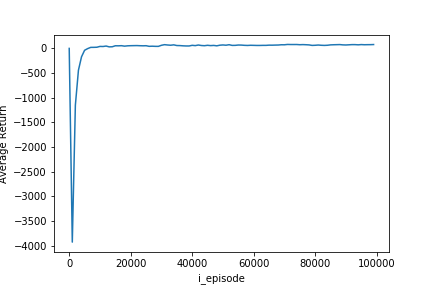
\includegraphics[scale = 0.7]{part5a.png}
\caption{Training curve}
\label{fig:part5_a}
\end{figure*}

The training curve shows that the average return keeps keeps increasing and converges to some small positive number after aroun $10,000$ episodes. To show this, we included some of the average return outputs below:
\begin{lstlisting}
Episode 0       Average return: -0.90
Episode 1000    Average return: -4519.30
Episode 2000    Average return: -1704.60
Episode 3000    Average return: -976.70
Episode 4000    Average return: -571.30
Episode 5000    Average return: -164.80
Episode 6000    Average return: -104.40
Episode 7000    Average return: 2.90
Episode 8000    Average return: 41.00
Episode 9000    Average return: 53.50
Episode 10000   Average return: 23.90
Episode 11000   Average return: 40.30
Episode 12000   Average return: 51.30
Episode 13000   Average return: 53.90
Episode 14000   Average return: 53.60
Episode 15000   Average return: 64.30
Episode 16000   Average return: 65.30
Episode 17000   Average return: 50.50
Episode 18000   Average return: 53.50
Episode 19000   Average return: 56.60
Episode 20000   Average return: 61.40
...
Episode 30000   Average return: 54.90
...
Episode 40000   Average return: 64.80
...
Episode 50000   Average return: 48.90
...
Episode 60000   Average return: 55.90
...
Episode 70000   Average return: 59.70
...
Episode 80000   Average return: 45.80
...
Episode 90000   Average return: 38.40
...
Episode 99000   Average return: 62.90
\end{lstlisting}

The choice of hyper-parameters are:
\begin{itemize}
    \item The learning rate $\alpha$ is $0.001$. This choice is based on moderate training speed without too much compromises on convergence.
    \item The reward for each action is defined above in Section 4b). We did not change these rewards because they are justified to be reasonable choices.
    \item The discount rate $\gamma$ is $1$, which means we are not discounting our reward. This is because when we defined the reward, the positive reward is always received when the game is ended (win). Therefore it does not make sense if we discount the reward, since we only care about if it wins the game or not (not how fast it can win the game).
    \item The maximum episode is defined to be $100,000$, this episode length is shown to be enough for the algorithm to converge.
    \item The neural network structure is same as that defined in Part 2. It has 27 input units, 64 units in a single hidden layer, and 9 output units. Such parameter is proven to be the optimal choice, based on the discussion below in Part 5b).
\end{itemize}

\clearpage

\subsubsection*{b)}
In order to optimize the number of hidden neurons in the policy, we tuned this parameter by training number of hidden nuerons = 5, 10, 30, 50, 70, 100, 150, 200. The results are shown below in Figure~\ref{fig:part5_b}


\begin{figure*}[!ht]
\centering

\begin{subfigure}{.35\textwidth}
\centering
  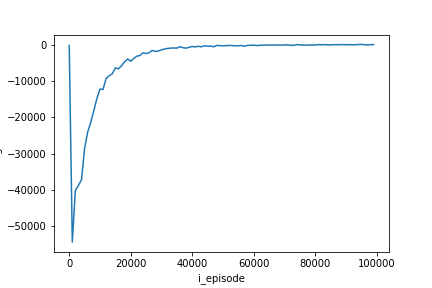
\includegraphics[width=1\linewidth]{part5b_5.png}
  \caption{5 hidden neurons}
  \label{fig:part5_b_5}
\end{subfigure}
\begin{subfigure}{.35\textwidth}
\centering
  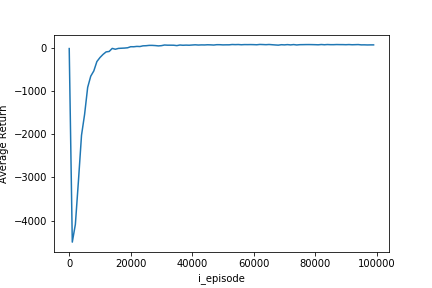
\includegraphics[width=1\linewidth]{part5b_10.png}
  \caption{10 hidden neurons}
  \label{fig:part5_b_10}
\end{subfigure}
\\
\begin{subfigure}{.35\textwidth}
\centering
  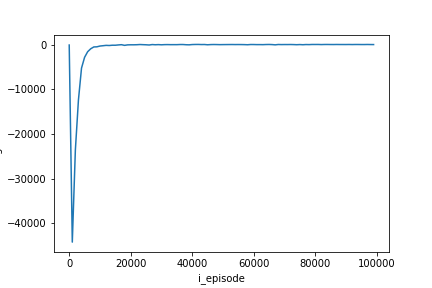
\includegraphics[width=1\linewidth]{part5b_30.png}
  \caption{30 hidden neurons}
  \label{fig:part5_b_30}
\end{subfigure}
\begin{subfigure}{.35\textwidth}
\centering
  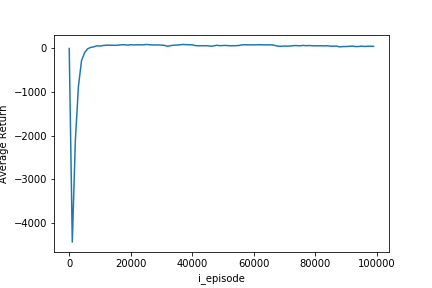
\includegraphics[width=1\linewidth]{part5b_50.png}
  \caption{50 hidden neurons}
  \label{fig:part5_b_50}
\end{subfigure}
\\
\begin{subfigure}{.35\textwidth}
\centering
  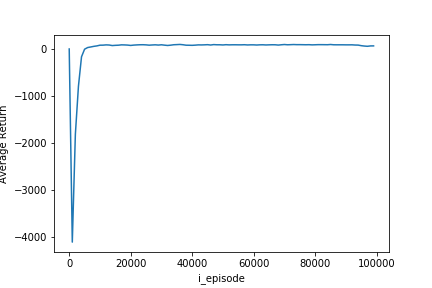
\includegraphics[width=1\linewidth]{part5b_70.png}
  \caption{70 hidden neurons}
  \label{fig:part5_b_70}
\end{subfigure}
\begin{subfigure}{.35\textwidth}
\centering
  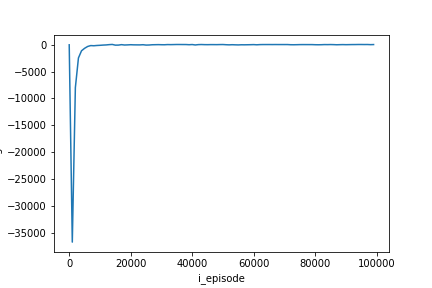
\includegraphics[width=1\linewidth]{part5b_100.png}
  \caption{100 hidden neurons}
  \label{fig:part5_b_100}
\end{subfigure}
\\
\begin{subfigure}{.35\textwidth}
\centering
  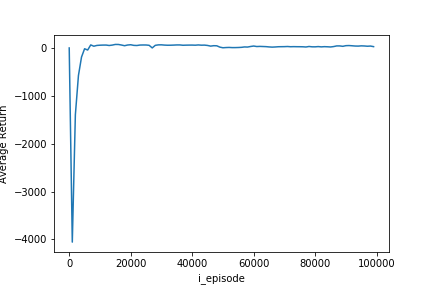
\includegraphics[width=1\linewidth]{part5b_150.png}
  \caption{150 hidden neurons}
  \label{fig:part5_b_150}
\end{subfigure}
\begin{subfigure}{.35\textwidth}
\centering
  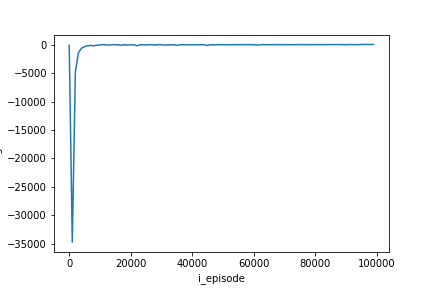
\includegraphics[width=1\linewidth]{part5b_200.png}
  \caption{200 hidden neurons}
  \label{fig:part5_b_200}
\end{subfigure}

\caption{Learning curves with different number of hidden layers}
\label{fig:part5_b}
\end{figure*}

Observe from above figure, we see that increasing the number of hidden neurons generally improves the performance, but with some unexpected behaviours if we have too many hidden neurons:
\begin{enumerate}
    \item The "plateau" occurs earlier (smaller episode) as the number of hidden neurons increases. This means that the policy converges faster to the optimal policy that gives a high positive average return. It also means that the policy learns to avoid invalid move more quickly.
    \item When the number of neurons is too large, the average return starts to fluctuate more. This fluctuation is very obvious in 100 hidden neurons, and also visible in 150 and 200 neurons.
    \item Additionally, a subtle observation is that the average return is higher/better for larger number of hidden neurons, as one can observe from the value in the y-axis. This means that models with more hidden neurons do "less worse" than model with less hidden neurons.
\end{enumerate}
To choose the appropriate structure for our model, we consider both the learning speed (i.e. how quickly the average return converges and how quickly it learns to not make invalid moves) and the computing efficiency. We also wish to avoid the possibility of having the big fluctuation at large number of hidden neurons. Therefore, we choose a number between $50$ and $70$, which is $64$. And it is proven in Part 5a) that this choice yield a reasonably good result. 


\subsubsection*{c)}
From Figure~\ref{fig:part5_a} we observe a sudden increase in average return at very early episodes. This is an indication of the policy starts to learn to not make invalid moves because we give a very high penalty for any invalid moves. Therefore, when the policy starts to try not make any invalid moves, we can observe a huge increase in average return, from large negative numbers to close to 0. 
\\
With the reference to sample output in Part 5a), we identified that the policy stops making invalid move around episode $7,000$ because episodes before $7,000$ has average return smaller than $-100$, which suggests that the policy is still making invalid moves in some cases (because the penalty for a game loss is $-100$, if the average return is smaller than $-100$, then it performed invalid moves.) Episode after $7,000$ has average return consistently higher than $-100$, which suggests that the policy learns to stop making invalid moves most of the time.


\subsubsection*{d)}
The results of 100 games with the learned policy played with \texttt{random} is listed in Table~\ref{table:part5d} below:

\begin{table}[!ht]
\centering
\caption{100 Game results played against random}
\label{table:part5d}
\begin{tabular}{|c|c|c|}
\hline
\textbf{\# Win} & \textbf{\# Lose} & \textbf{\# Tie} \\ \hline
90              & 6                & 4               \\ \hline
\end{tabular}
\end{table}

To illustrate the strategy learned by the policy, five sample game is included below:

\begin{lstlisting}
Game No.1 begin!
...
.x.
.o.
====
..x
.x.
.oo
====
..x
.x.
xoo
====
Game No.1 finished! Result: win 
\end{lstlisting}

\begin{lstlisting}
Game No.3 begin!
..o
.x.
...
====
x.o
.xo
...
====
x.o
.xo
..x
====
Game No.3 finished! Result: win 
\end{lstlisting}

\begin{lstlisting}
Game No.7 begin!
.o.
.x.
...
====
.ox
ox.
...
====
xox
ox.
o..
====
xox
ox.
o.x
====
Game No.7 finished! Result: win 
\end{lstlisting}

\begin{lstlisting}
Game No.24 begin!
...
ox.
...
====
x.o
ox.
...
====
x.o
ox.
x.o
====
xxo
oxo
x.o
====
Game No.24 finished! Result: lose 
\end{lstlisting}

\begin{lstlisting}
Game No.38 begin!
x..
o..
...
====
xo.
ox.
...
====
xo.
ox.
..x
====
Game No.38 finished! Result: win 
\end{lstlisting}



From above examples, the policy we trained tends to have the following strategy:
\begin{itemize}
    \item The first step is either placing at position (2,2), the middle position, such as in Game No. 1, 3, 7, 24; or place at position (1,1), which is the left upper corner, such as in Game No.38
    \item If the first step is placing at position (2,2), then, the strategy is to place next 'x' in (1,3) and try form (1,3)-(2,2)-(3,1) to win the game, such as Game No.1. Or, the strategy is to place next 'x' in (1,1) and form (1,1)-(2,2)-(3,3) to win the game, if the position (1,3) or (3,3) is occupied by 'o', such as in Game No.3, No.7.
    \item However, the above strategy may not work, for example, in Game No. 24, the strategy fails because the opponent 'o' are placed in both (1,3) and (3,3) positions, blocking the winning strategy.
    \item If the first step is placing at position (1,1), then the winning strategy seems to be have 'x' in (1,1)-(2,2)-(3,3) to win the game, such as in Game No.38.
\end{itemize}

\end{homeworkProblem}
\clearpage


%----------------------------------------------------------------------------------------
%	PROBLEM 6
%----------------------------------------------------------------------------------------

\begin{homeworkProblem}
\noindent \textit{Win Rate over Episodes}
\\[10pt]
The win / lose / tie rate throughout training episodes is shown below in Figure~\ref{fig:part6}
\begin{figure*}[!ht]
\centering
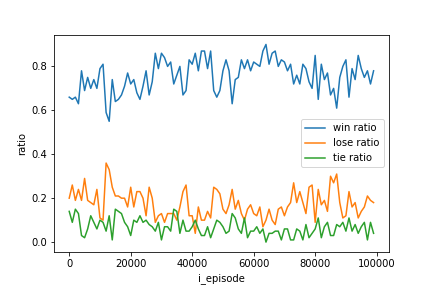
\includegraphics[scale = 0.7]{part6.png}
\caption{Win / Lose / Tie rate at different training episodes}
\label{fig:part6}
\end{figure*}

From the figure above, we observe the following:
\begin{itemize}
    \item The winning ratio is consistently higher than the lose and tie ratio. This suggests the strategy is consistently better than opponent with random move.
    \item The winning ratio has an observable increase at the beginning stage of the training, from episode 0 to around episode 8000. This suggests that our training has let the policy learned some particular strategies that can lead to a higher winning probability at the initial stage. Also, this learning speed is fairly quick: only takes about 8000 episodes.
    \item Because of the increase in winning ratio, the losing and tie ratio decrease at the early stage of training.
    \item Then, three ratios seem to be fluctuating - the winning ratio fluctuate between 70\% to 90\%. And the losing and tie ratio fluctuates correspondingly. But it is important to note that the magnitude of fluctuation decreases as the episode increases. This means that the policy is trying to learn a strategy that gives a consistent result.
    \item Overall, the win ratio is about 80\%, lose and tie ratio is about 10\% each at the later episodes, with some fluctuation.
    
\end{itemize}

\end{homeworkProblem}
\clearpage




%----------------------------------------------------------------------------------------
%	PROBLEM 7
%----------------------------------------------------------------------------------------

\begin{homeworkProblem}
\noindent \textit{First Move Distribution over Episodes}
\\[10pt]
The learned distribution over the first move in shown as a heat map below in Figure~\ref{fig:part7_learned}

\begin{figure*}[!ht]
\centering
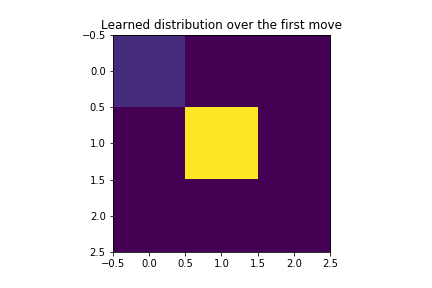
\includegraphics[scale = 0.7]{part7_fullyTrained.png}
\caption{Learned distribution over the first move}
\label{fig:part7_learned}
\end{figure*}

From the heat map above, it is evident that our learned strategy tends to put its first move at center (2,2) with highest probability, but sometimes it also place its first move in the left upper corner (1,1). The strategy almost never place its first move in other positions.
\\
This distribution makes sense because:
\begin{itemize}
    \item The strategy should learn a fairly deterministic first move, in this case, it only places first move in location (2,2) and (1,1).
    \item The center location (2,2) has the highest probability. This makes sense because the center position leads to 4 possible winning routes, namely the two diagonals, vertical and horizontal routes; whereas other positions only lead to at most 3 possible winning routes.
    \item The strategy sometimes places its first move in location (1,1). This maybe caused by the fact that placing first move in location (1,1) can lead to similar outcome (i.e. the winning probability, or the reward) as placing in location (2,2).
    \item Intuitively, if humans were playing this game, most people will place the first move either in the center position or in the corner, which aligns with our trained strategy.
    \item Finally, these possible two moves for the first move maybe one of the underlying results why the average return graph in Part 6 has some level of fluctuation, because different first move may lead to different outcomes.
\end{itemize}

\clearpage

The distribution over the first move in different positions with respect to different episodes is shown below in Figure~\ref{fig:part7_each}

\begin{figure*}[!ht]
\centering

\begin{subfigure}{.32\textwidth}
\centering
  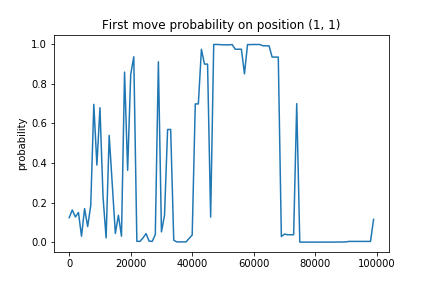
\includegraphics[width=1\linewidth]{part7_position_1,1.png}
  \caption{Position (1,1)}
  \label{fig:part7_11}
\end{subfigure}
\begin{subfigure}{.32\textwidth}
\centering
  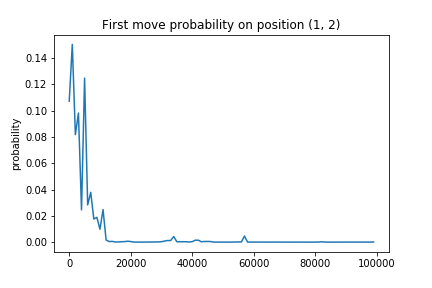
\includegraphics[width=1\linewidth]{part7_position_1,2.png}
  \caption{Position (1,2)}
  \label{fig:part7_12}
\end{subfigure}
\begin{subfigure}{.32\textwidth}
\centering
  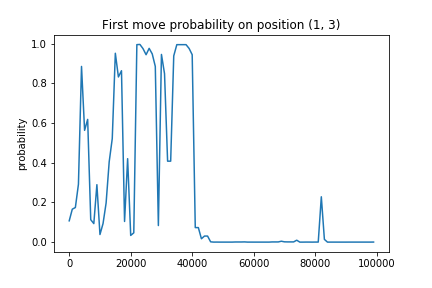
\includegraphics[width=1\linewidth]{part7_position_1,3.png}
  \caption{Position (1,3)}
  \label{fig:part7_13}
\end{subfigure}
\\
\begin{subfigure}{.32\textwidth}
\centering
  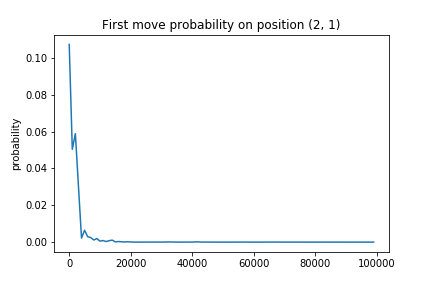
\includegraphics[width=1\linewidth]{part7_position_2,1.png}
  \caption{Position (2,1)}
  \label{fig:part7_21}
\end{subfigure}
\begin{subfigure}{.32\textwidth}
\centering
  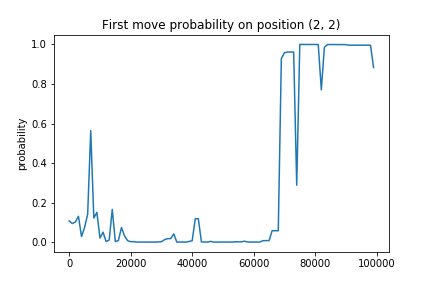
\includegraphics[width=1\linewidth]{part7_position_2,2.png}
  \caption{Position (2,2)}
  \label{fig:part7_22}
\end{subfigure}
\begin{subfigure}{.32\textwidth}
\centering
  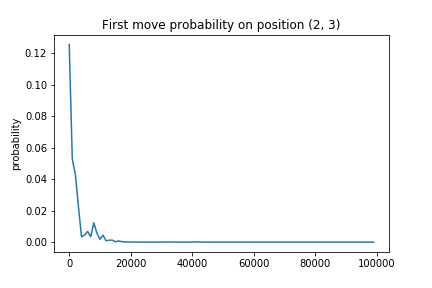
\includegraphics[width=1\linewidth]{part7_position_2,3.png}
  \caption{Position (2,3)}
  \label{fig:part7_23}
\end{subfigure}
\\
\begin{subfigure}{.32\textwidth}
\centering
  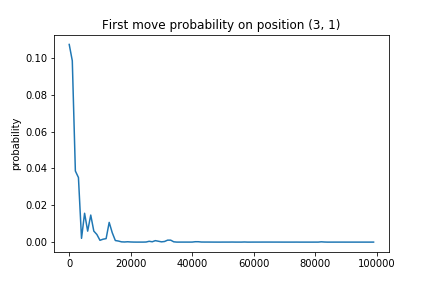
\includegraphics[width=1\linewidth]{part7_position_3,1.png}
  \caption{Position (3,1)}
  \label{fig:part7_31}
\end{subfigure}
\begin{subfigure}{.32\textwidth}
\centering
  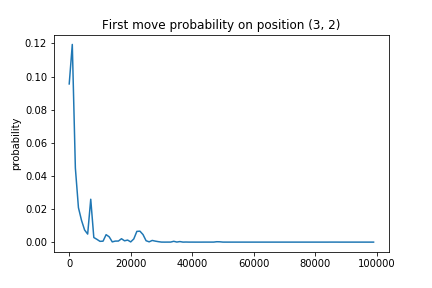
\includegraphics[width=1\linewidth]{part7_position_3,2.png}
  \caption{Position (3,2)}
  \label{fig:part7_32}
\end{subfigure}
\begin{subfigure}{.32\textwidth}
\centering
  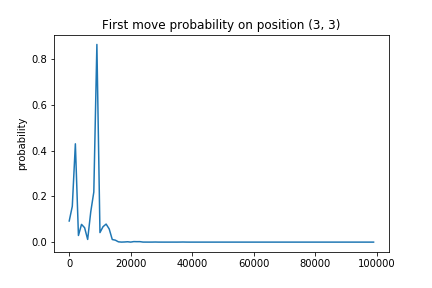
\includegraphics[width=1\linewidth]{part7_position_3,3.png}
  \caption{Position (3,3)}
  \label{fig:part7_33}
\end{subfigure}

\caption{Learning curves with different number of hidden layers}
\label{fig:part7_each}
\end{figure*}

From above figure, we can see that the probability distribution aligns with our previous discussion on the learned distribution on first move. In particular, we observe the following:
\begin{itemize}
    \item The probability of first move placed in location (1,2), (1,3), (2,1), (2,3), (3,1), (3,2) (3,3) reaches close to 0 at later episode, although some location may have some fluctuation. This suggests that the policy has learned not to place its first move in these seven locations.
    \item The probability of first move placed in location (2,2) reaches near to 100\% at later stage of the episode, the suggests that the policy has learned to place its first move in the center location.
    \item It is important to note that near the end, close to 100000 episodes, the probability of placing first move at location (2,2) decreases and the probability at location (1,1) increases. This contributes to over final distributed probability demonstrated earlier in Figure~\ref{fig:part7_learned}, where the strategy is to place most of its first move in location (2,2), and sometimes in (1,1). This could be due to a possible fluctuation, or maybe the strategy is exploring that placing first move in (1,1) may lead to higher average return.
\end{itemize}

\end{homeworkProblem}
\clearpage

%----------------------------------------------------------------------------------------
%	PROBLEM 8
%----------------------------------------------------------------------------------------
\begin{homeworkProblem}
\noindent \textit{Limitations}
\\[10pt]
Although the learned policy performs reasonably well against a random policy, we defined some mistakes our agent makes:
\begin{enumerate}
    \item The agent fails to stop an obvious lose from happening. In other words, it fails to place 'x' in a position such that it will block three opponent 'o' strike, which let the opponent wins the game. For example, in Game No.66 shown below, the agent should place its third 'x' in position (2,1) to prevent losing. However, it fails to do so, and eventually loses the game.
    \item The agent fails to observe a winning move, if it does not follow the original wining strategy learned (The winning strategy is discussed Part 5d)). For example, in Game No.91 below, the agent should place an 'x' in position (2,3) at its fourth step to win the game. However, it failed to do so because the winning route (1,3)-(2,3)-(3,3) is not a winning strategy learned by the policy. Therefore, the agent seems to make random moves and lead to a tie game.
\end{enumerate}

\begin{lstlisting}
Game No.66 begin!
x..
.o.
...
====
x.x
.oo
...
====
xox
.oo
..x
====
xox
ooo
x.x
====
Game No.66 finished! Result: lose 
\end{lstlisting}

\begin{lstlisting}
Game No.91 begin!
.o.
.x.
...
====
.ox
.x.
o..
====
oox
.x.
o.x
====
oox
xxo
o.x
====
oox
xxo
oxx
====
Game No.91 finished! Result: tie 
\end{lstlisting}

\end{homeworkProblem}
\clearpage
%----------------------------------------------------------------------------------------

\end{document}